\documentclass{boi2014-lt}

\usepackage{enumitem}
\usepackage{todonotes}
\usepackage{wrapfig}

\renewcommand{\DayNum}{2}
\renewcommand{\TaskCode}{demarcation}
\renewcommand{\TaskName}{Demarkacija}
\renewcommand{\TaskVersion}{1.2}

\newcommand{\constant}[1]{{\tt #1}}

\begin{document}
    \begin{wrapfigure}{r}{3cm}
        \vspace{-24pt}
        \includegraphics[width=3cm]{\TaskCode.jpeg}
    \end{wrapfigure}

    Karalius Baitazaras ilgai ir teisingai valdė Baitopijos salą. Tačiau po
    staigios jo mirties jo sūnūs dvyniai -- Bitonas ir Baitonas -- niekaip
    negalėjo sutarti, kuris iš jų turėtų paveldėti sostą. Jie nusprendė
    padalinti salą į dvi provincijas, kurias valdytų nepriklausomai.
 
    Stačiakampyje žemėlapyje Baitopija yra $N$ viršūnių turintis daugiakampis.
    Visos daugiakampio kraštinės yra lygiagrečios žemėlapio kraštinėms, o
    tarp kiekvienos gretimų daugiakampio kraštinių poros yra status kampas. Jokia
    daugiakampio kraštinė nekerta ir neliečia jokios kitos kraštinės, išskyrus
    gretimų kraštinių galus.

    Bitonas ir Baitonas nori padalinti salą į du kongruenčius daugiakampius
    viena atkarpa, kuri būtų salos daugiakampio viduje ir būtų lygiagreti
    žemėlapio kraštinei. (Du daugiakampiai yra kongruentūs jeigu vienas iš jų
    gali būti transformuotas į kitą kokia nors atspindžio, posūkio ir poslinkio
    operacijų kombinacija.) Visų daugiakampio viršūnių ir ieškomos dalinančios
    atkarpos galų koordinatės yra sveikieji skaičiai.
 
    Karaliaus sūnūs prašo jūsų patikrinti, ar toks salos padalinimas yra
    įmanomas.

    \Task
    Duotai salos formai nustatykite, ar ji gali būti padalinta horizontalia arba
    vertikalia atkarpa į du kongruenčius daugiakampius. Jeigu toks padalinimas
    egzistuoja, raskite taip salą dalinančią atkarpą.

    \Input
    Pirmoje eilutėje yra vienas sveikasis skaičius $N$ -- daugiakampio viršūnių
    skaičius. Iš kitų $N$ eilučių $i$-ojoje yra tarpais atskirta sveikųjų
    skaičių pora $X_i$ ir $Y_i$ ($0 \le X_i, Y_i \le 10^9$) -- $i$-osios
    viršūnės koordinatės.
    
    Viršūnės pateiktos iš eilės, t.~y. daugiakampio kraštinės yra atkarpos
    $(X_1,Y_1) - (X_2,Y_2)$, $(X_2,Y_2) - (X_3,Y_3)$, \ldots,
    $(X_{N-1},Y_{N-1}) - (X_N,Y_N)$ ir $(X_N,Y_N) - (X_1,Y_1)$. Be to, bet
    kurios dvi iš eilės einančios atkarpos yra viena kitai statmenos.

    \Output
    Jūsų programa turėtų išvesti vieną eilutę. Jeigu įmanoma padalinti salą į du
    kongruenčius daugiakampius horizontalia arba vertikalia atkarpa, kurios galų
    koordinatės yra $(x_1, y_1)$ ir $(x_2, y_2)$, išspausdinkite $4$ tarpais
    atskirtus sveikuosius skaičius $x_1$, $y_1$, $x_2$ ir $y_2$. Jiems turėtų
    galioti bent viena iš lygybių $x_1 = x_2$ arba $y_1 = y_2$. Ši atkarpa
    turėtų būti daugiakampio viduje ir tik jos galai turėtų liesti daugiakampio
    ribas.

    Jeigu neįmanoma rasti tinkamo salos padalinimo, išveskite vieną žodį
    \constant{NO}.
    
    \pagebreak

    \Examples
    \example
    {
        10 \newline
        0 0 \newline
        1 0 \newline
        1 1 \newline
        3 1 \newline
        3 5 \newline
        2 5 \newline
        2 3 \newline
        1 3 \newline
        1 2 \newline
        0 2
    }
    {
        1 2 3 2
    }
    {
        Atkreipkite dėmesį, kad {\tt 3 2 1 2} irgi yra teisingas sprendinys.
        
        \begin{center}
            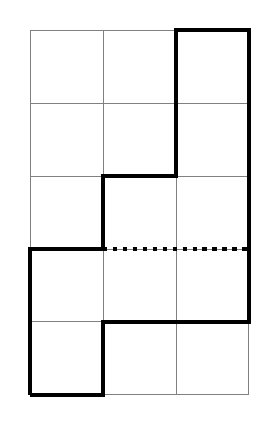
\begin{tikzpicture}[scale=0.9266625]
            \draw[help lines] (0,0) grid (3,5);
            \draw[ultra thick] (0,0) -- (1,0) -- (1,1) -- (3,1) -- (3,5) --
                         (2,5) -- (2,3) -- (1,3) -- (1,2) -- (0,2) -- (0,0);
            \draw[ultra thick,dotted] (1,2) -- (3,2);
            \end{tikzpicture}
        \end{center}
    }

    \example
    {
        6 \newline
        0 0 \newline
        1 0 \newline
        1 1 \newline
        2 1 \newline
        2 2 \newline
        0 2
    }
    {
        NO
    }
    {
        Šiuo atveju padalinti salą į du kongruenčius daugiakampius yra neįmanoma.
        \begin{center}
            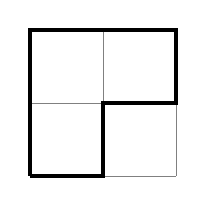
\begin{tikzpicture}[scale=0.9266625]
            \draw[help lines] (0,0) grid (2,2);
            \draw[ultra thick] (0,0) -- (1,0) -- (1,1) --
                         (2,1) -- (2,2) -- (0,2) -- (0,0);
            \end{tikzpicture}
        \end{center}
    }

    \Scoring

    \begin{description}
        \item[Dalinė užduotis Nr. 1 (12 taškų).] $4 \le N \le 100\ 000$.
            Bet kuri horizontali arba vertikali tiesė, kuri kerta daugiakampį,
            dalina jį į lygiai dvi dalis.
        \item[Dalinė užduotis Nr. 2 (15 taškų).] $4 \le N \le 200$
        \item[Dalinė užduotis Nr. 3 (23 taškai).] $4 \le N \le 2\ 000$
        \item[Dalinė užduotis Nr. 4 (50 taškų).] $4 \le N \le 100\ 000$
    \end{description}

    \Constraints

    \begin{description}
        \item[Laiko limitas:] 0,5 s.
        \item[Atminties limitas:] 256 MB.
    \end{description}

\end{document}
